\documentclass{article}
% translate with >> pdflatex -shell-escape <file>

\usepackage{pgfplots}
\pgfplotsset{compat=newest}

\pagestyle{empty}

\begin{document}
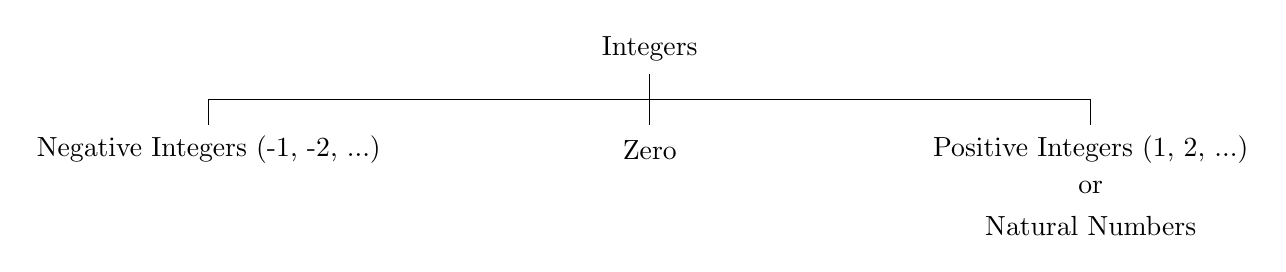
\begin{tikzpicture}[scale=1.6]%
   \draw (0,0) -- (7,0);
   \draw (3.5, -0.2) -- (3.5, 0.2);
   \draw (3.5, 0.4) node {Integers};
   \draw (3.5, -0.4) node {Zero};
   \draw (0, -0.2) -- (0, 0);
   \draw (7, -0.2) -- (7, 0);
   \draw (0, -0.4) node {Negative Integers (-1, -2, ...)};
   \draw (7, -0.4) node {Positive Integers (1, 2, ...)};
   \draw (7, -0.7) node {or};
   \draw (7, -1) node {Natural Numbers};
\end{tikzpicture}%
\end{document}
